\documentclass[11pt,openany]{article}

\usepackage{mathtools, commath}
% Packages for formatting
\usepackage[margin=1in]{geometry}
\usepackage{fancyhdr}
\usepackage{enumerate}
\usepackage{graphicx}
\usepackage{kotex}
\usepackage{arydshln} % Include this package
\usepackage{bbding}
\usepackage{amsmath}
\usepackage{amsthm}
\usepackage[dvipsnames,table]{xcolor}
\usepackage{amssymb, amsfonts}
\usepackage{wasysym}
\usepackage{footnote}
\usepackage{tablefootnote}
\usepackage{arydshln} % Include this package
% Fonts
\usepackage[T1]{fontenc}
\usepackage[utf8]{inputenc}
\usepackage{newpxtext,newpxmath}
\usepackage{sectsty}

% Define colors
\definecolor{TealBlue1}{HTML}{0077c2}
\definecolor{TealBlue2}{HTML}{00a5e6}
\definecolor{TealBlue3}{HTML}{b3e0ff}
\definecolor{TealBlue4}{HTML}{00293c}
\definecolor{TealBlue5}{HTML}{e6f7ff}

\definecolor{thmcolor}{RGB}{231, 76, 60}
\definecolor{defcolor}{RGB}{52, 152, 219}
\definecolor{lemcolor}{RGB}{155, 89, 182}
\definecolor{corcolor}{RGB}{46, 204, 113}
\definecolor{procolor}{RGB}{241, 196, 15}

\usepackage{color,soul}
\usepackage{soul}
\newcommand{\mathcolorbox}[2]{\colorbox{#1}{$\displaystyle #2$}}
\usepackage{cancel}
\newcommand\crossout[3][black]{\renewcommand\CancelColor{\color{#1}}\cancelto{#2}{#3}}
\newcommand\ncrossout[2][black]{\renewcommand\CancelColor{\color{#1}}\cancel{#2}}

\usepackage{hyperref}
\usepackage{booktabs}

% Chapter formatting
\definecolor{titleTealBlue}{RGB}{0,53,128}
\usepackage{titlesec}
\titleformat{\section}
{\normalfont\sffamily\Large\bfseries\color{titleTealBlue!100!gray}}{\thesection}{1em}{}
\titleformat{\subsection}
{\normalfont\sffamily\large\bfseries\color{titleTealBlue!50!gray}}{\thesubsection}{1em}{}

%Tcolorbox
\usepackage[most]{tcolorbox}
\usepackage{multirow}
\usepackage{multicol}

\usepackage[linesnumbered,ruled]{algorithm2e}
\usepackage{algpseudocode}
\usepackage{setspace}
\SetKwComment{Comment}{/* }{ */}
\SetKwProg{Fn}{Function}{:}{end}
\SetKw{End}{end}
\SetKw{DownTo}{downto}

% Define a new environment for algorithms without line numbers
\newenvironment{algorithm2}[1][]{
	% Save the current state of the algorithm counter
	\newcounter{tempCounter}
	\setcounter{tempCounter}{\value{algocf}}
	% redefine the algorithm numbering (remove prefix)
	\renewcommand{\thealgocf}{}
	\begin{algorithm}
	}{
	\end{algorithm}
	% Restore the algorithm counter state
	\setcounter{algocf}{\value{tempCounter}}
}

\usepackage{adjustbox}
% Header and footer formatting
\pagestyle{fancy}
\fancyhead{}
\fancyhf{}
\rhead{\textcolor{TealBlue2}{\large\textbf{기대수(기초부터 대학원 수학까지 시리즈) 3기}}}%\rule{3cm}{0.4pt}}
\lhead{\textcolor{TealBlue2}{\large\textbf{수학의 즐거움, Enjoying Math}}}
% Define footer
%\newcommand{\footer}[1]{
%\begin{flushright}
%	\vspace{2em}
%	\includegraphics[width=2.5cm]{school_logo.jpg} \\
%	\vspace{1em}
%	\textcolor{TealBlue2}{\small\textbf{#1}}
%\end{flushright}
%}
%\rfoot{\large Department of Information Security, Cryptogrphy and Mathematics, Kookmin Uni.\includegraphics[height=1.5cm]{school_logo.jpg}}
\fancyfoot{}
\fancyfoot[C]{-\thepage-}

\usepackage{tcolorbox}
\tcbset{colback=white, arc=5pt}

\definecolor{axiomcolor}{HTML}{a88bfa}
\definecolor{defcolor}{RGB}{52, 152, 219}
\definecolor{procolor}{RGB}{241, 196, 15}
\definecolor{thmcolor}{RGB}{231, 76, 60}
\definecolor{lemcolor}{RGB}{155, 89, 182}
\definecolor{corcolor}{RGB}{46, 204, 113}
\definecolor{execolor}{RGB}{90, 128, 127}

% Define a new command for the custom tcolorbox
\newcommand{\axiombox}[2][]{%
	\begin{tcolorbox}[colframe=axiomcolor, title={\color{white}\bfseries #1}]
		#2
	\end{tcolorbox}
}

\newcommand{\defbox}[2][]{%
	\begin{tcolorbox}[colframe=defcolor, title={\color{white}\bfseries #1}]
		#2
	\end{tcolorbox}
}

\newcommand{\lembox}[2][]{%
	\begin{tcolorbox}[colframe=lemcolor, title={\color{white}\bfseries #1}]
		#2
	\end{tcolorbox}
}

\newcommand{\probox}[2][]{%
	\begin{tcolorbox}[colframe=procolor, title={\color{white}\bfseries #1}]
		#2
	\end{tcolorbox}
}

\newcommand{\thmbox}[2][]{%
	\begin{tcolorbox}[colframe=thmcolor, title={\color{white}\bfseries #1}]
		#2
	\end{tcolorbox}
}

\newcommand{\corbox}[2][]{%
	\begin{tcolorbox}[colframe=corcolor, title={\color{white}\bfseries #1}]
		#2
	\end{tcolorbox}
}



\usepackage{amsthm}

% Define custom theorem styles
\newtheoremstyle{dotless} % Name of the style
{3pt} % Space above
{3pt} % Space below
{\itshape} % Body font
{} % Indent amount
{\bfseries} % Theorem head font
{} % Punctuation after theorem head
{2.5mm} % Space after theorem head
{} % Theorem head spec

\newtheoremstyle{definitionstyle} % Name of the style
{3pt} % Space above
{3pt} % Space below
{} % Body font
{} % Indent amount
{\bfseries} % Theorem head font
{.} % Punctuation after theorem head
{2.5mm} % Space after theorem head
{} % Theorem head spec

% Applying custom styles
\theoremstyle{dotless}
\newtheorem{theorem}{Theorem} % Theorem environment with section-wise numbering
\newtheorem{proposition}[theorem]{Proposition} % Theorem environment with section-wise numbering
\newtheorem{lemma}[theorem]{Lemma} % Lemma shares the counter with theorem
\newtheorem{corollary}[theorem]{Corollary} % Corollary shares the counter with theorem

\theoremstyle{definitionstyle}
\newtheorem*{observation}{\textcolor{Magenta}{Observation}}
\newtheorem{definition}{Definition} % Definition shares the counter with theorem
\newtheorem{example}{Example} % Example shares the counter with theorem
\newtheorem{exercise}{Exercise} % Example shares the counter with theorem
\newtheorem{remark}{Remark} % Remark shares the counter with theorem
\newtheorem*{note}{Note}

\newtheorem*{definition*}{Definition} % Definition shares the counter with theorem
\newtheorem*{example*}{Example} % Example shares the counter with theorem
\newtheorem*{exercise*}{\textcolor{violet}{Exercise}} % Example shares the counter with theorem
\newtheorem*{remark*}{Remark} % Remark shares the counter with theorem


\usepackage{tikz}
\usepackage{tikz-cd}
\usepackage{tikz-3dplot}
\usepackage{pgfplots}
\pgfplotsset{compat=newest} % Adjust to your version of pgfplots
\def\Circlearrowleft{\ensuremath{%
		\rotatebox[origin=c]{180}{$\circlearrowleft$}}}
\def\Circlearrowright{\ensuremath{%
		\rotatebox[origin=c]{180}{$\circlearrowright$}}}
\def\CircleArrowleft{\ensuremath{%
		\reflectbox{\rotatebox[origin=c]{180}{$\circlearrowleft$}}}}
\def\CircleArrowright{\ensuremath{%
		\reflectbox{\rotatebox[origin=c]{180}{$\circlearrowright$}}}}
\usetikzlibrary{
	3d, % For 3D drawing
	angles,
	arrows,
	arrows.meta,
	backgrounds,
	bending,
	calc,
	decorations.pathmorphing,
	decorations.pathreplacing,
	decorations.markings,
	fit,
	matrix,
	patterns,
	patterns.meta,
	positioning,
	quotes,
	shadows,
	shapes,
	shapes.geometric,
	tikzmark
}
\tikzset{
	% single mid‐path arrow
	mid arrow/.style={
		decoration={
			markings,
			mark=at position 0.5 with {\arrow{Stealth[scale=1.2]}}
		},
		postaction={decorate},
	},
	% style for field arrows
	field arrow/.style={
		-{Stealth[scale=1.0]},
		thick,
		blue!70!black,
	},
}
\newcommand{\ie}{\textnormal{i.e.}}
\newcommand{\rsa}{\mathsf{RSA}}
\newcommand{\rsacrt}{\mathsf{RSA}\textendash\mathsf{CRT}}
\newcommand{\inv}[1]{#1^{-1}}

%New Command
%\newcommand{\set}[1]{\left\{#1\right\}}
\newcommand{\N}{\mathbb{N}}
\newcommand{\Z}{\mathbb{Z}}
\newcommand{\Q}{\mathbb{Q}}
\newcommand{\R}{\mathbb{R}}
\newcommand{\cR}{\mathcal{R}}
\newcommand{\C}{\mathbb{C}}
\newcommand{\F}{\mathbb{F}}
\newcommand{\nbhd}{\mathcal{N}}
\newcommand{\Log}{\operatorname{Log}}
\newcommand{\Arg}{\operatorname{Arg}}
\newcommand{\pv}{\operatorname{P.V.}}

\newcommand{\of}[1]{\left( #1 \right)} 
%\newcommand{\abs}[1]{\left\lvert #1 \right\rvert}
%\newcommand{\norm}[1]{\left\| #1 \right\|}

\newcommand{\sol}{\textcolor{magenta}{\bf Sol}}
\newcommand{\conjugate}[1]{\overline{#1}}

\newcommand{\res}{\operatorname{res}}
\DeclareMathOperator*{\Res}{\operatorname{Res}}

%\renewcommand{\Re}{\operatorname{Re}}
%\renewcommand{\Im}{\operatorname{Im}}

\newcommand{\cyclic}[1]{\langle #1 \rangle}
\newcommand{\uniform}{\overset{\$}{\leftarrow}}
\newcommand{\xmark}{\textcolor{red}{\XSolidBrush}}
\newcommand{\vmark}{\textcolor{green!75!black}{\CheckmarkBold}}

\newcommand{\gen}[1]{\langle #1 \rangle}
\newcommand{\Gen}[1]{\left\langle #1 \right\rangle}

\newcommand{\img}[1]{\text{Img}(#1)}
\newcommand{\Img}[1]{\text{Img}\left(#1\right)}
\newcommand{\preimg}[1]{\text{Img}^{-1}(#1)}
\newcommand{\Preimg}[1]{\text{Img}^{-1}\left(#1\right)}

\newcommand{\relation}{\mathrel{\mathcal{R}}}
\newcommand{\injection}{\rightarrowtail}
\newcommand{\surjection}{\twoheadrightarrow}
\newcommand{\id}{\textnormal{id}}

\newcommand{\eqclass}[1]{\left[#1\right]}

% Define custom colors for O and X
\newcommand{\yes}{\textcolor{blue}{\bf \fullmoon}}
\newcommand{\no}{\textcolor{red}{\bf \texttimes}}

\DeclarePairedDelimiter\ceil{\lceil}{\rceil}
\DeclarePairedDelimiter\floor{\lfloor}{\rfloor}
%\renewcommand{\floor}[#1]{\lfloor #1\rfloor}
%\newcommand{\Floor}[#1]{\left\lfloor #1\right\rfloor}
%\newcommand{\ceil}[#1]{\lceil #1\rceil}
%\newcommand{\Ceil}[#1]{\left\lceil #1\right\rceil}

\newcommand{\topology}{\mathscr{T}}
\newcommand{\sequence}[1]{\langle #1\rangle}
\renewcommand{\vec}[1]{\mathbf{#1}}
\renewcommand{\Re}{\operatorname*{Re}}
\renewcommand{\Im}{\operatorname*{Im}}
\setstretch{1.25}

%\usepackage{background}
%\backgroundsetup{
%	scale=3,
%	color=gray!20,
%	opacity=0.3,
%	angle=45,
%	contents={\Huge \sffamily Ji, Yong-hyeon}
%}
\begin{document}
\pagenumbering{arabic}
\begin{center}
	\huge\textbf{Abstract Algebra II}\\
	\vspace{0.5em}
	\large{Ji, Yong-hyeon}\\
%	\large{\ttfamily \url{https://github.com/Hacker-Code-J}}\\
	\vspace{0.5em}
	\normalsize{\today}\\
\end{center}

\noindent 
We cover the following topics in this note.
\begin{itemize}
	\item Group Action
	\item Cayley Theorem
	\item Normal Subgroups
	\item Normality of the Kernel
\end{itemize}
\hrule\vspace{12pt}
%\tableofcontents
\begin{center}
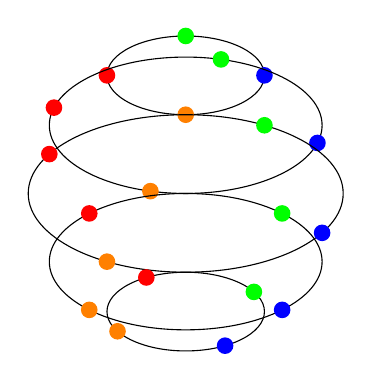
\begin{tikzpicture}[scale=2]
% Define the viewing tilt angle (in degrees) and its sine/cosine for reuse
\def\tiltAngle{30}%
\pgfmathsetmacro{\cosphi}{cos(\tiltAngle)}%
\pgfmathsetmacro{\sinphi}{sin(\tiltAngle)}%
% Loop over two rows (start angles 0 and 180 degrees for first frame in each row)
%\foreach \row/\startAng in {0/0,1/180} {%
	\foreach \row/\startAng in {1/180} {%
% In each row, loop over 6 columns (frames)
%	\foreach \col in {0,...,5} {%
	\foreach \col in {0} {%
		% Calculate the rotation angle for this frame (adds 30° per step in the row)
		\pgfmathsetmacro{\globalAng}{\startAng + 30*\col}%
		% Shift coordinate system for this frame’s position in the grid
		\begin{scope}[shift={(\col*3, -\row*3)}]%
		% Draw the sphere (5 horizontal orbit circles with sample points)
		\foreach \i in {1,...,5} {%
			% Latitude for orbit i (i=1 top, i=5 bottom): 60°, 30°, 0°, -30°, -60°
			\pgfmathsetmacro{\lat}{60 - (\i-1)*30}%
			\pgfmathsetmacro{\r}{cos(\lat)}% horizontal radius of orbit
			\pgfmathsetmacro{\z}{sin(\lat)}% vertical center of orbit
			\pgfmathsetmacro{\offAng}{(\i-1)*15}% initial offset angle for this orbit’s points
			% Draw orbit circle as an ellipse (wireframe latitude)
			\draw [thin, black] (0, {\z * \cosphi}) ellipse ({\r} and {\r * \sinphi});
			% Draw four colored points on this orbit, at 0°, 90°, 180°, 270° around (plus offset and global rotation)
			\foreach \angOff/\clr in {0/red, 90/green, 180/blue, 270/orange} {%
					\pgfmathsetmacro{\ptAng}{\globalAng + \offAng + \angOff}%
					\fill [\clr] ({\r * cos(\ptAng)}, {-\r * \sinphi * sin(\ptAng) + \z * \cosphi}) circle[radius=1.5pt];
			}%
		}%
		\end{scope}%
	}%
}%
\end{tikzpicture}
\end{center}
\def\acts{\curvearrowright}
%\newpage
\vspace{20pt}
\defbox[Group Action]{\begin{definition*}
Let \( (G,\ast) \) be a group and let \( X\neq\varnothing \). A \textbf{(left) group action} of \( G \) on \( X \) is a function \[
\cdot : G \times X \to X,\quad (g, x) \mapsto g \cdot x
\]
satisfying the followings: for all \( g, h \in G \) and all \( x \in X \),
\begin{enumerate}[(i)]
	\item (Identity)\; \( e \cdot x = x \), where \( e \in G \) is the identity element of \( G \);
	\item (Compatibility)\; \( (g\ast h) \cdot x = g \cdot (h \cdot x) \).
\end{enumerate}
The pair \( (X, \cdot) \) (or simply \( X \) ) is then called a \( G \)-set.
\end{definition*}}
\begin{note}[Notation]
If a group \( G \) acts on a set \( X \), one commonly writes: $G \curvearrowright X$.
\end{note}
\begin{remark*}
	A right group action of \( G \) on \( X \) is a function $
	\cdot : X \times G \to X,\quad (x, g) \mapsto x \cdot g$ 
	satisfying: \begin{enumerate}[(i)]
		\item \( x \cdot e = x \) for all \( x \in X \);
		\item \( (x \cdot g) \cdot h = x \cdot (gh) \) for all \( g, h \in G \), \( x \in X \).
	\end{enumerate}
\end{remark*}

\newpage
\begin{example*}[Scalar Multiplication on a Vector Space]
	Let \( \mathbb{F} \) be a field, and let \( X = \mathbb{F}^n \) be the \( n \)-dimensional vector space over \( \mathbb{F} \). Consider the multiplicative group of nonzero scalars in \( \mathbb{F} \): \[
	G = (\F^\times, \times),\quad\text{where}\; \F^\times=\mathbb{F} \setminus \{0\}.
	\] We define an action \( G \curvearrowright X \) by scalar multiplication:
	\[
	\fullfunction{\cdot}{\F^\times\times\F^n}{\F^n}{(\lambda,\vec{v})}{\lambda\cdot\vec{v}},
	\] where the product \( \lambda\cdot \vec{v} \) is defined componentwise. Then \begin{enumerate}[(i)]
		\item \( 1 \cdot \vec{v} = \vec{v} \) for all \( \vec{v} \in \mathbb{F}^n \).
		\item \( (\lambda\mu) \cdot \vec{v} = \lambda \cdot (\mu \cdot \vec{v}) \) for all \( \lambda, \mu \in \mathbb{F}^\times \), \( \vec{v} \in \mathbb{F}^n \).
	\end{enumerate}
	\begin{center}
	\begin{tikzpicture}[scale=1]
		\coordinate (O) at (0,0);
		\coordinate (v) at (2,1);
		\coordinate (lv) at (3,1.5); % assuming \lambda=1.5
		\draw[->] (-0.5,0) -- (4,0) node[right] {$x$};
		\draw[->] (0,-0.5) -- (0,3) node[above] {$y$};
		\draw[->, thick, blue]  (O) -- (v);
		\fill[blue] (v)  circle (2pt) node[above right] {$\vec v = (v_1,v_2)$};
		\draw[dashed, -Latex] (5,2) to node[above] {$\F^\times\acts\F^2$} (9,2) ;
		\begin{scope}[xshift=10cm]
			\coordinate (O) at (0,0);
			\coordinate (v) at (2,1);
			\coordinate (lv) at (3,1.5); % assuming \lambda=1.5
			\draw[->] (-0.5,0) -- (4,0) node[right] {$x$};
			\draw[->] (0,-0.5) -- (0,3) node[above] {$y$};
			\draw[->, thick, red]   (O) -- (lv);
			\fill[red] (lv) circle (2pt) node[above right] {$\lambda\vec v=(\lambda v_1,\lambda v_2)$};
		\end{scope}
	\end{tikzpicture}
	\end{center}
\end{example*}
\vfill
\begin{example*}[Conjugation Action on the Group Itself]
Let \( G \) be any group, and consider \( X = G \). Define an action of \( G \) on itself by conjugation: \[
G \curvearrowright G, \quad (g, x) \mapsto g \cdot x := g\ast x\ast g^{-1}.
\] Then \begin{enumerate}[(i)]
	\item \( e \cdot x = e\ast x\ast e^{-1} = x \) for all \( x \in G \).
	\item Note that \begin{align*}
		(g\ast h) \cdot x &= (g\ast h)\ast x\ast (g\ast h)^{-1} \\
		&= (g\ast h)\ast x\ast (h^{-1}\ast g^{-1})\\
		&= g\ast (h\ast x\ast h^{-1})\ast g^{-1}\\
		&= g\ast (h\cdot x)\ast g^{-1}\\
		&=g \cdot (h \cdot x).
	\end{align*} Thus, this is a left group action.
%	Its **orbits** are the **conjugacy classes** in \( G \), and the **stabilizer** of \( x \in G \) is the **centralizer**: \[
%	\operatorname{Stab}_G(x) = \{ g \in G \mid gxg^{-1} = x \} = C_G(x).
%	\]
%	The kernel of this action is the **center** \( Z(G) = \{ g \in G \mid gx = xg \text{ for all } x \in G \} \).
\end{enumerate}
\end{example*}

\newpage
\begin{example*}[Trivial \( G \)-Set]
Let \( G \) be any group and define the set \( X = \{x\} \), a singleton. Define the action
\[
G \curvearrowright X, \quad (g,x)\mapsto g \cdot x := x \quad \text{for all } g \in G.
\] This is the \textbf{trivial action}, where every group element acts as the identity on \( X \):
\begin{enumerate}[(i)]
	\item \( e \cdot x = x \).
	\item \( (g\ast h) \cdot x = x = g \cdot (h \cdot x) \).
\end{enumerate}
%This is the unique action of \( G \) on a singleton, and it appears naturally when defining constant \( G \)-sets or fixed points. 
%in more general actions.
\end{example*}
\vfill
\begin{example*}[Action on Coset Space \( G/H \)]
Let $(G,\ast)$ be a group, and let \( H \leq G \). Let \( X = G/H \) be the set of left cosets of \( H \) in \( G \), \ie,
\[
X = G/H = \{ gH \mid g \in G \}.
\] Define an action \[
G \curvearrowright G/H, \quad (g, aH) \mapsto (ga)H.
\] This is well-defined because if \( a_1H = a_2H \), then \( a_1^{-1}a_2 \in H \), so: $
g a_1 H = g a_2 H.$. Since \begin{enumerate}[(i)]
	\item \( e \cdot aH = aH \);
	\item \( (gh) \cdot aH = g \cdot (h \cdot aH) \).
\end{enumerate}
%this is a \textbf{transitive action}.
%and the stabilizer of the coset \( eH \in G/H \) is \( H \) itself. 
%This action reflects the **quotient structure** of \( G \) by \( H \), and is fundamental in the construction of **homogeneous spaces** and **induced representations**.
\end{example*}
\vfill
\probox[Group Elements Act as Permutations]{\begin{proposition*}
Let \( G \) be a group action on a set \( X \) via a left action \( G \curvearrowright X \), given by \( (g, x) \mapsto g \cdot x \). Then for each \( g \in G \), the map
\[
\sigma_g : X \to X, \quad x \mapsto g \cdot x
\]
is one-to-one and onto. {\color{gray!50} That is, \( \sigma_g \in \operatorname{Sym}(X) \), the group of all permutations of \( X \).}
\end{proposition*}}
\begin{proof}
	TBA
	%To show that \( \sigma_g \) is bijective, observe that its inverse is \( \sigma_{g^{-1}} \), since for all \( x \in X \):
	%
	%\[
	%\sigma_{g^{-1}}(\sigma_g(x)) = g^{-1} \cdot (g \cdot x) = (g^{-1}g) \cdot x = e \cdot x = x,
	%\]
	%\[
	%\sigma_g(\sigma_{g^{-1}}(x)) = g \cdot (g^{-1} \cdot x) = (gg^{-1}) \cdot x = e \cdot x = x.
	%\]
	%
	%Hence, \( \sigma_g \) is invertible with inverse \( \sigma_{g^{-1}} \), and thus \( \sigma_g \) is bijective.
\end{proof}

\newpage
\thmbox[Group Actions Induce Permutation Representations]{\begin{theorem*}
Let \( G \) be a group action on a set \( X \) via a left group action $G \curvearrowright X, \quad (g, x) \mapsto g \cdot x$. For each \( g \in G \), define the bijection \( \sigma_g : X \to X \) by $
\sigma_g(x) := g \cdot x$. Then the map \[
\phi: G \to \operatorname{Sym}(X), \quad g\mapsto \sigma_g,
\] is a \textbf{group homomorphism} from \( G \) to the symmetric group \( \operatorname{Sym}(X) \).
In other words, for all \( g, h \in G \), \[
\phi(g\ast h) = \sigma_{g\ast h}=\sigma_g\circ\sigma_h= \phi(g) \circ \phi(h).
\]
\end{theorem*}}
\begin{remark*}
	A group action $G\acts X$ is equivalent to a group homomorphism $G\to \operatorname{Sym}(X)$, i.e., a \textbf{permutation representation} of $G$.
\end{remark*}
\begin{proof}
	TBA
%### **Proof.**
%
%Let \( g, h \in G \), and let \( x \in X \). By the definition of \( \sigma_g \) and the group action axioms,
%
%\[
%\sigma_{gh}(x) = (gh) \cdot x = g \cdot (h \cdot x) = \sigma_g(\sigma_h(x)) = (\sigma_g \circ \sigma_h)(x).
%\]
%
%Since this equality holds for all \( x \in X \), it follows that \( \sigma_{gh} = \sigma_g \circ \sigma_h \). Therefore, \( \phi \) is a homomorphism.
\end{proof}

\thmbox[Cayley Theorem]{\begin{theorem*} 
Let \(G\) be a group. Consider the action of \(G\) on itself by left multiplication.  For each \(g\in G\), define  
\[
\sigma_g \;:\; G \;\longrightarrow\; G,\qquad x\;\mapsto\;g\cdot x.
\]  
Then the map  
\[
\phi \;:\; G \;\longrightarrow\;\operatorname{Sym}(G),\qquad g\;\mapsto\;\sigma_g
\]  
is an injective group homomorphism (group monomorphism).  In particular,  \[
\phi(G)\simeq G
\quad\text{and}\quad
\phi(G)\le\operatorname{Sym}(G).
\]
\end{theorem*}}
\begin{proof}
	TBA
%#### Proof sketch.  
%1. **Homomorphism.**  For all \(g,h\in G\) and \(x\in G\),  
%\[
%\phi(gh)(x)
%= \sigma_{gh}(x)
%= (gh)\,x
%= g\,(h\,x)
%= \sigma_g\bigl(\sigma_h(x)\bigr)
%= \bigl(\sigma_g\circ\sigma_h\bigr)(x),
%\]  
%hence \(\phi(gh)=\sigma_g\circ\sigma_h=\phi(g)\phi(h)\).
%
%2. **Injectivity.**  If \(\phi(g)=\mathrm{id}_G\), then for every \(x\in G\),  
%\[
%g\,x = \sigma_g(x) = x,
%\]  
%so in particular \(g\cdot e = e\) forces \(g=e\).  Thus \(\ker\phi=\{e\}\) and \(\phi\) is injective.
\end{proof}

\newpage
\section*{Normal Subgroups}
\begin{observation}
	Consider $4\Z\leq \Z$. Then \[
	\Z/4\Z=\set{0+4\Z,1+4\Z,2+4\Z,3+4\Z}=\set{[0],[1],[2],[3]}.
	\] \begin{itemize}
		\item $[0]+[1]=(0+4\Z)+(1+4\Z)\overset{\text{def.}}{=}(0+1)+4\Z=1+4\Z=[1]$.
		\item $[1]+[2]=(1+4\Z)+(2+4\Z)\overset{\text{def.}}{=}(1+2)+4\Z=3+4\Z=[3]$.
		\item $[1]+[3]=(2+4\Z)+(3+4\Z)\overset{\text{def.}}{=}(1+3)+4\Z=4+4\Z=0+4\Z= [0]$.
	\end{itemize}
\end{observation}
\vspace{20pt}
\probox[Existence of the Quotient Group]{\begin{proposition*}
	Let \((G,\ast)\) be a group and let \(H\leq G\) be a subgroup.  Define a binary operation $\boxast$ on the set of left cosets \(G/H\) by  \[
	(g\ast H)\boxast (g'\ast H) \;=\;(g\ast g')\ast H
	\] where $g,g'\in G$.
	Then this operation is well-defined 
%	(and makes \(G/H\) into a group) 
	if and only if \[
	g\ast h\ast g^{-1}\;\in\;H.
	\]  for all $g\in G$, $h\in H.$
\end{proposition*}}
\begin{proof}
	TBA
%\begin{itemize}
%	\item[($\Rightarrow$)] Let $g\in G$ and $h\in H$. Then \begin{align*}
%		h\ast g^{-1}\in H\implies g\ast H=g(h)
%	\end{align*}
%	\item[($\Leftarrow$)]
%\end{itemize}
\end{proof}

\newpage
\defbox[Normal Subgroup]{\begin{definition*}
	Let \((G,\ast)\) be a group and let \(H\leq G\). We say that $H$ is \textbf{normal} in $G$, written \[
	H\trianglelefteq G,
	\] if $g\ast h\ast g^{-1}\in H$ for any $g\in G$ and $h\in H$.
\end{definition*}}
\begin{remark*}
The set of (left) cosets $G/H$ be a well-defined group structure via \[
(g\ast H)\boxast (k\ast H) = (g\ast k)\ast H,
\] making $G/H$ the quotient group of $G$ by $H$.
\end{remark*}

\vfill
\probox[Equivalent Definitions of Normal Subgroup]{\begin{proposition*}
Let \((G,\ast)\) be a group and let \(H\leq G\). The Following Are Equivalent: 
\begin{enumerate}[\normalfont (1)]
	\item[\normalfont (1)\footnote{Terminology and Notation}] $H$ is normal in $G$, \ie, $H\trianglelefteq G$;
	\item[\normalfont (2)\footnote{(Elementwise Conjugation)}] $g\ast h\ast g^{-1}\in H$ for all $g\in G$, $h\in H$;
	\item[\normalfont (3)\footnote{(Conjugation Invariance)}] $g\ast H\ast g^{-1}=H$ for all $g\in G$;
	\item[\normalfont (4)\footnote{(Coset Equality)}] $g\ast H=H\ast g$ for all $g\in G$.
\end{enumerate}
\end{proposition*}}
\begin{proof}
\begin{enumerate}
	\item[] \hspace{-1cm} ((2)$\Rightarrow$(3)) TBA
	\item[] \hspace{-1cm} ((3)$\Rightarrow$(4)) TBA
	\item[] \hspace{-1cm} ((4)$\Rightarrow$(2)) TBA
\end{enumerate}
\end{proof}

\newpage
\thmbox[Normality of Kernel]{\begin{theorem*} 
Let $\phi: (G,\ast) \;\longrightarrow\; (H,\ast')$ be a group homomorphism, and define its kernel by \[
	\ker\phi \;=\;\set{\,g\in G : \phi(g)=e_H}\,.  
\] Then \(\ker\phi\) is a normal subgroup of \(G\); that is, $\ker\phi \;\trianglelefteq\; G$.
\end{theorem*}}
\begin{proof}
	Since \(\phi\) is a homomorphism, for every \(g\in G\) and every \(k\in\ker\phi\) we have  
	\[
	\phi\bigl(g\ast k\ast g^{-1}\bigr)
	=\phi(g)\ast'\phi(k)\ast'\phi(g)^{-1}
	=\phi(g)\ast'e_H\ast'\phi(g)^{-1}
	=e_H,
	\] so \(g\ast k\ast g^{-1}\in\ker\phi\). Thus,  
	\[
	g\ast(\ker\phi)\ast g^{-1} \;=\; \ker\phi
	\quad\forall\,g\in G,
	\]  
	i.e.\ \(\ker\phi\) is invariant under conjugation and hence normal in \(G\).  
\end{proof}


%**Explaining why kernel is normal**
%
%The user is asking why the kernel of a group homomorphism is normal, specifically in terms of elementwise conjugation, conjugation invariance, and coset equality.
%
%The kernel consists of elements mapping to the identity, and for any element $g$ in $G$ and $k$ in the kernel, if we conjugate $k$ by $g$ (i.e., $gkg^{-1}$), we still get an element in the kernel. This is based on the property of homomorphisms, ensuring closure under conjugation.
%
%Aligning these perspectives: for quotient groups, we need kernels to be normal so the structure is well-defined on cosets; conjugation invariance means inner automorphisms fix it; coset equality simply means cosets can swap places, confirming normality.
%
%
%Thought for 5 seconds
%
%
%A good way to see “why the kernel of any group homomorphism is normal” is to translate that fact into each of your three favorite languages:
%
%---
%
%## 1. Elementwise conjugation
%
%> **“For every $k\in\ker\phi$ and every $g\in G$, the conjugate $gkg^{-1}$ is still in $\ker\phi$.”**
%
%* **Reason:**
%
%$$
%\phi(gkg^{-1})
%\;=\;
%\phi(g)\,\phi(k)\,\phi(g)^{-1}
%\;=\;
%\phi(g)\,e\,\phi(g)^{-1}
%\;=\;
%e.
%$$
%
%Therefore $gkg^{-1}\in\ker\phi$.  That exactly says “$\ker\phi$” is **closed under conjugation** by arbitrary $g$.
%
%---
%
%## 2. Conjugation‐invariance (inner automorphisms)
%
%> **“Every inner automorphism of $G$ fixes $\ker\phi$ set-wise.”**
%
%* An inner automorphism is $I_g\!:x\mapsto g\,x\,g^{-1}$.
%* We just showed $I_g(\ker\phi)\subseteq\ker\phi$.  But $I_{g^{-1}}$ is its inverse map, so in fact $I_g(\ker\phi)=\ker\phi$.
%* In other words, **no matter how you ‘twist’ $G$ by conjugation, the kernel sits exactly in the same place**.  That is the hallmark of a normal subgroup.
%
%---
%
%## 3. Coset‐equality
%
%> **“Left‐cosets of $\ker\phi$ agree with right‐cosets, so $G/\!\ker\phi$ is well defined as a group of cosets.”**
%
%* Because $g\,(\ker\phi)\,g^{-1} = \ker\phi$, you get
%
%$$
%g\,(\ker\phi)
%= (g\,\ker\phi\,g^{-1})\,g
%= \ker\phi\,g.
%$$
%* Thus for every $g$,
%
%$$
%g\,\ker\phi \;=\;\ker\phi\,g,
%$$
%
%so **left** and **right** cosets coincide.  Equivalently, you can multiply cosets $(a\,\ker\phi)\cdot(b\,\ker\phi)=(ab)\,\ker\phi$ without ambiguity.
%
%---
%
%### Why this matters in each context
%
%| Context                           | Normality via kernel                                                                                                                                                                       |
%| --------------------------------- | ------------------------------------------------------------------------------------------------------------------------------------------------------------------------------------------ |
%| **Constructing the quotient**     | If $\ker\phi$ weren’t invariant under conjugation, the product of cosets would depend on choices of representatives.  Normality makes $G/\!\ker\phi$ into a well‐defined group.            |
%| **Group actions / automorphisms** | Kernels are exactly the points fixed by all images $\phi(g)$.  Conjugation invariance means those “fixed points” form a symmetric, $G$-stable subset.                                      |
%| **Checking by generators**        | If you know a presentation of $\ker\phi$, you just verify each generator $k$ satisfies $gkg^{-1}\in\langle\text{generators}\rangle$.  Again, that’s the same elementwise‐conjugation test. |
%
%---
%
%**Bottom line:**
%
%> No matter which viewpoint you take—elementwise conjugation, invariance under inner automorphisms, or coset‐equality—the defining property of a normal subgroup is exactly that its elements “get carried into itself by conjugation.”  Since the kernel of a homomorphism is by definition sent to the identity, and conjugation in the image can only carry the identity to itself, the kernel must be invariant under every conjugation in $G$.

\newpage
\begin{illustration}
\ \\
\adjustbox{scale=.75, center}{
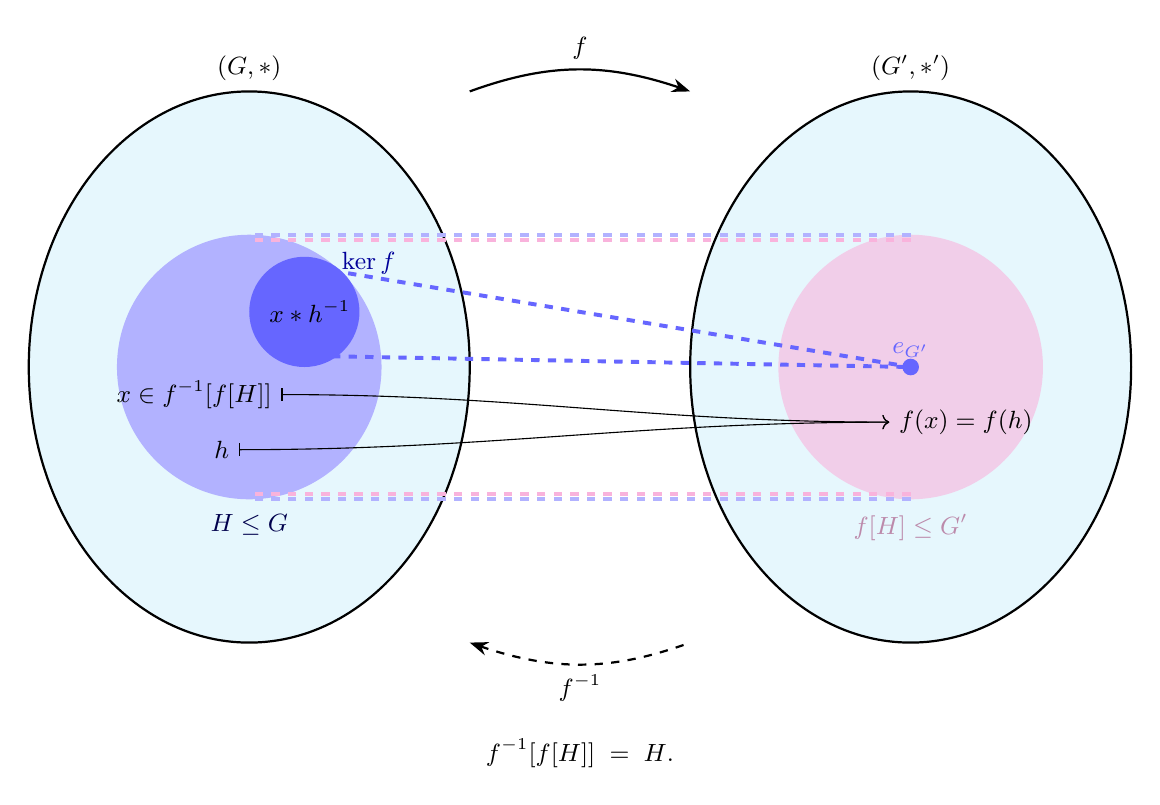
\begin{tikzpicture}[every node/.style={font=\small}, scale=1.4]
	% Domain G
	\filldraw[cyan!10] (-3,0) ellipse (2 and 2.5);
	\draw[thick]       (-3,0) ellipse (2 and 2.5) node[above=3.5cm] {$(G,\ast)$};
	% Subgroup H inside G
	\begin{scope}
		\clip (-3,0) ellipse (2 and 2.5);
		\fill[blue!30] (-3,0) circle (1.2) node[blue!30!black, below=1.75cm] {$H\leq G$};
	\end{scope}
	%\node[blue!60!black] at (-4.4,-1.8) {$H\leq G$};
	
	% Codomain G'
	\filldraw[cyan!10] (3,0) ellipse (2 and 2.5);
	\draw[thick]       (3,0) ellipse (2 and 2.5) node[above=3.5cm] {$(G',\ast')$};
	% Image f[H] inside G'
	\begin{scope}
		\clip (3,0) ellipse (2 and 2.5);
		\fill[magenta!30,opacity=0.6] (3,0) circle (1.2) node[magenta!60!black, below=1.75cm] {$f[H]\leq G'$};
	\end{scope}
	%\node[magenta!60!black] at (4.5,-1.8) {$f[H]\le G'$};
	
	% Forward arrow f
	\draw[-Stealth, thick] (-1,2.5) to[bend left=20] node[above] {$f$} (1,2.5);
	% Backward arrow f^{-1}
	\draw[Stealth-, dashed, thick] (-1,-2.5) to[bend right=20] node[below] {$f^{-1}$} (1,-2.5);
	
	% Label the equality of sets f^{-1}(f[H]) = H
	\node at (0,-3.5) {\(\displaystyle f^{-1}[f[H]]\;=\;H\).};
	
	\draw[dashed, blue!30, line width=.5mm] (3,1.195) to (-3,1.195);
	\draw[dashed, blue!30, line width=.5mm] (3,0-1.195) to (-3,-1.195);
	\draw[dashed, magenta!30, line width=.5mm] (3,1.155) to (-3,1.155);
	\draw[dashed, magenta!30, line width=.5mm] (3,0-1.155) to (-3,-1.155);
	
	\node (x) at (-3.5,-.25) {$x\in f^{-1}[f[H]]$};
	\node (h) at (-3.25,-.75) {$h$};
	\node (fx) at (3.5,-.5) {$f(x)=f(h)$};
	\draw[|->, bend angle=45, out=0, in=180] (x) to (fx);
	\draw[|->, bend angle=45, out=0, in=180] (h) to (fx);

	% Kernel inside H
	\begin{scope}
		\clip (-3,0) ellipse (2 and 2.5);
		\fill[blue!60] (-2.5,0.5) circle (0.5) node[blue!60!black, above right=.5cm] {$\ker f$};
	\end{scope}
	%\node[blue!60!black] at (-2.1,1.3) {$\ker f$};
	\node at (-2.45,.5) {$x\ast h^{-1}$};
	\draw[dashed, blue!60, line width=.5mm] (-2.4,.9) to (3,0);
	\draw[dashed, blue!60, line width=.5mm] (-2.4,.1) to (3,0);
	\filldraw[blue!60] (3,0) circle (2pt) node[above] {$e_{G'}$};
\end{tikzpicture}}
\end{illustration}
\thmbox[Preimage of the Image of a Subgroup]{\begin{theorem*} 
	Let $f: (G,\ast) \to (G',\ast')$ be a group homomorphism, and let $H\leq G$ such that  \[
	\{\,g\in G:f(g)=e_{G'}\}=\ker f\subseteq H.
	\] Then \[
	f^{-1}[f[H]]=H,
	\] with $f[H] = \{ f(h) \mid h \in H \}$ and $f^{-1}[f[H]] = \{ g \in G \mid f(g) \in f[H] \}$.
\end{theorem*}}
\begin{proof}
	Suppose that $\ker f\subseteq H\leq G$. We NTS that $f^{-1}[f[H]]=H$: \begin{itemize}
		\item[($\supseteq$)] $h\in H\implies
		f(h)\in f[H]\implies h\in f^{-1}[f[H]]$.
		\item[($\subseteq$)] Let $x\in f^{-1}[f[H]]$. Then $f(x)\in f[H]$; that is, \[
		\exists h\in H\quad\text{such that}\quad f(h)=f(x).
		\] Thus, \[
		f(x\ast h^{-1})=f(x)\ast 'f(h)^{-1}=f(x)\ast'f(x)^{-1}=e_{G'},
		\] so $x\ast h^{-1}\in\ker f$. Since $\ker f\subseteq H$, we have \[
		x=(x\ast h^{-1})\ast h\in H,
		\] and hence $f^{-1}[f[H]]\subseteq H$.
	\end{itemize}
\end{proof}

\newpage
\thmbox[]{\begin{theorem*}
Let $\phi\colon G\;\longrightarrow\;G'$ be a surjective homomorphism of groups.  Define two collections: \[
\mathcal{S}
\;=\;
\bigl\{\,H\subseteq G : \ker\phi\subseteq H\le G\bigr\},
\qquad
\mathcal{T}
\;=\;
\bigl\{\,H'\subseteq G' : H'\le G'\bigr\}.
\] Then the map \[
\Phi\colon\mathcal{S}\;\longrightarrow\;\mathcal{T},
\qquad
\Phi(H)\;=\;\phi(H)
\] is a bijection.  Its inverse is \[
\Phi^{-1}\colon\mathcal{T}\;\longrightarrow\;\mathcal{S},
\qquad
\Phi^{-1}(H')\;=\;\phi^{-1}(H').
\] Moreover, \[
H\trianglelefteq G\iff\phi(H)\trianglelefteq G'.
\]
\end{theorem*}}
%\begin{remark*}
%\ \begin{enumerate}
%	\item (Inclusion)\; For $H_1,H_2\in\mathcal{S}$,\; $H_1\subseteq H_2\iff
%	\phi(H_1)\subseteq\phi(H_2)$.
%	\item (Normality)\;
%	$H\trianglelefteq G$ if and only if $\phi(H)\trianglelefteq G'$.
%	\item (Index)\; If $H_1\subseteq H_2$ in $\mathcal{S}$, then $[H_2 : H_1]=\bigl[\phi(H_2) : \phi(H_1)\bigr]$.
%\end{enumerate}
%\end{remark*}
\begin{proof}
%**Theorem (Correspondence Theorem for Groups).**
%Let
%$$
%\phi\colon G\;\longrightarrow\;G'
%$$
%
%be a **surjective** homomorphism of groups.  Define
%
%$$
%\mathcal{S}
%=\{\,H\le G : \ker\phi\subseteq H\}, 
%\quad
%\mathcal{T}
%=\{\,H'\le G'\}.
%$$
%
%Then the map
%
%$$
%\Phi\colon\mathcal{S}\;\longrightarrow\;\mathcal{T},
%\qquad
%\Phi(H)=\phi(H)
%$$
%
%is a bijection, with inverse
%
%$$
%\Phi^{-1}\colon\mathcal{T}\;\longrightarrow\;\mathcal{S},
%\qquad
%\Phi^{-1}(H')=\phi^{-1}(H').
%$$
%
%Moreover, for $H_1,H_2\in\mathcal{S}$ and $H'\in\mathcal{T}$:
%
%1. $H_1\subseteq H_2\iff \phi(H_1)\subseteq\phi(H_2)$.
%2. $H\triangleleft G\iff \phi(H)\triangleleft G'$.
%3. If $H_1\subseteq H_2$, then $[H_2:H_1]=[\phi(H_2):\phi(H_1)].$
%
%---
%
%### Proof
%
%#### 1. Well‐definedness of $\Phi$ and $\Phi^{-1}$
%
%* If $H\in\mathcal{S}$, then $\ker\phi\subseteq H\le G$.  The image of a subgroup under any homomorphism is a subgroup of the codomain, so $\phi(H)\le G'$.  Hence $\Phi(H)\in\mathcal{T}$.
%
%* If $H'\in\mathcal{T}$, then $H'\le G'$.  Thus
%
%$$
%\phi^{-1}(H') 
%= \{\,g\in G : \phi(g)\in H'\}
%$$
%
%is a subgroup of $G$ containing $\ker\phi$.  Hence $\Phi^{-1}(H')\in\mathcal{S}$.
%
%#### 2. $\Phi^{-1}\circ\Phi=\mathrm{id}_{\mathcal{S}}$
%
%Let $H\in\mathcal{S}$.  Then $\ker\phi\subseteq H$, and by the Lemma
%
%$$
%\phi^{-1}\bigl(\phi(H)\bigr)
%= H.
%$$
%
%Thus $\Phi^{-1}(\Phi(H))=H$.
%
%#### 3. $\Phi\circ\Phi^{-1}=\mathrm{id}_{\mathcal{T}}$
%
%Let $H'\in\mathcal{T}$.  Since $\phi$ is surjective,
%
%$$
%\phi\bigl(\phi^{-1}(H')\bigr)
%= H'.
%$$
%
%Hence $\Phi(\Phi^{-1}(H'))=H'$.
%
%Combining (2) and (3) shows $\Phi$ is a bijection with inverse $\Phi^{-1}$.
%
%---
%
%#### 4. Order‐preservation
%
%If $H_1,H_2\in\mathcal{S}$ with $H_1\subseteq H_2$, then $\phi(H_1)\subseteq\phi(H_2)$ by functoriality of images.  Conversely, if $\phi(H_1)\subseteq\phi(H_2)$, apply $\phi^{-1}$ to get
%
%$$
%H_1
%= \phi^{-1}\bigl(\phi(H_1)\bigr)
%\subseteq \phi^{-1}\bigl(\phi(H_2)\bigr)
%= H_2.
%$$
%
%---
%
%#### 5. Normality correspondence
%
%* If $H\triangleleft G$, then for every $g'\in G'$ choose $g\in G$ with $\phi(g)=g'$.  For any $x'\in\phi(H)$ write $x'= \phi(h)$.  Then
%
%$$
%g'\,x'\,(g')^{-1}
%= \phi(g)\,\phi(h)\,\phi(g)^{-1}
%= \phi\bigl(g\,h\,g^{-1}\bigr)\in \phi(H),
%$$
%
%since $g\,h\,g^{-1}\in H$.  Thus $\phi(H)\triangleleft G'$.
%
%* Conversely, if $\phi(H)\triangleleft G'$, then for every $g\in G$ and $h\in H$ we have
%
%$$
%\phi\bigl(g\,h\,g^{-1}\bigr)
%= \phi(g)\,\phi(h)\,\phi(g)^{-1}
%\in \phi(H).
%$$
%
%Hence $g\,h\,g^{-1}\in \phi^{-1}\bigl(\phi(H)\bigr)=H$, so $H\triangleleft G$.
%
%---
%
%#### 6. Index equality
%
%Let $H_1\subseteq H_2$ in $\mathcal{S}$.  Since $\ker\phi\subseteq H_1\subseteq H_2$, the restriction
%
%$$
%\phi|_{H_2}\colon H_2\;\to\;\phi(H_2)
%$$
%
%is surjective with kernel
%$\ker(\phi|_{H_2})=H_2\cap\ker\phi=\ker\phi$.  By the First Isomorphism Theorem,
%
%$$
%H_2 / \ker\phi
%\;\cong\;
%\phi(H_2),
%\qquad
%H_1 / \ker\phi
%\;\cong\;
%\phi(H_1).
%$$
%
%Since $\ker\phi\subseteq H_1\subseteq H_2$, the subgroup $H_1/\ker\phi$ sits inside $H_2/\ker\phi$, and indices satisfy
%
%$$
%[H_2 : H_1]
%= [\,H_2/\ker\phi : H_1/\ker\phi\,]
%= [\,\phi(H_2) : \phi(H_1)\,].
%$$
%
%This completes the proof of the Correspondence Theorem. 

\end{proof}


\vfill
\begin{thebibliography}{9}
	\bibitem{abstract_algebra_d}
	수학의 즐거움, Enjoying Math. ``수학 공부, 기초부터 대학원 수학까지, 23. 추상대수학 (d) 군 작용과 케일리-정리 group action and Cayley theorem'' YouTube Video, 29:20. Published 
	October 23, 2019. URL: \url{https://www.youtube.com/watch?v=5SQfrH83HfA&t=1040s}.
	\bibitem{abstract_algebra_e}
	수학의 즐거움, Enjoying Math. ``수학 공부, 기초부터 대학원 수학까지, 24. 추상대수학 (e) 정규부분군의 정의 def of normal subgroups'' YouTube Video, 23:00. Published 
	October 25, 2019. URL: \url{https://www.youtube.com/watch?v=3UJILZr4CNo}.
	\bibitem{abstract_algebra_f}
	수학의 즐거움, Enjoying Math. ``수학 공부, 기초부터 대학원 수학까지, 25. 추상대수학 (f) 정규부분군간의 1-1 대응 관계 1-1 correspondence of normal subgroups'' YouTube Video, 29:02. Published 
	October 26, 2019. URL: \url{https://www.youtube.com/watch?v=na0YYLJLWeQ}.
\end{thebibliography}

\newpage
\appendix
\section{Appendices}
\subsection{The Rotation Action of $\mathbb{S}^1$ on $\mathbb{S}^2$}
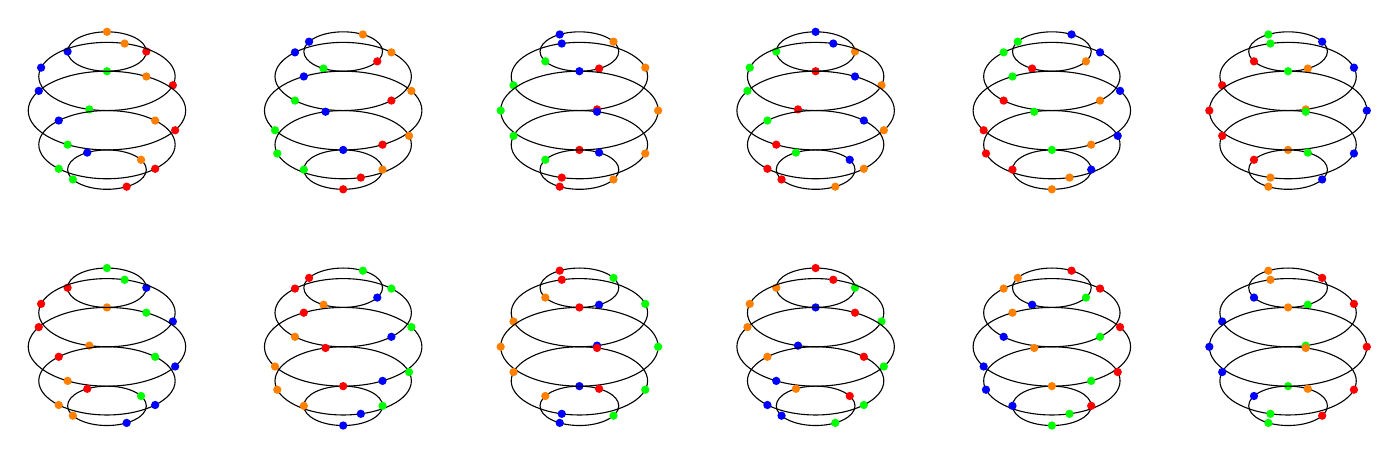
\begin{tikzpicture}
	% Define the viewing tilt angle (in degrees) and its sine/cosine for reuse
	\def\tiltAngle{30}%
	\pgfmathsetmacro{\cosphi}{cos(\tiltAngle)}%
	\pgfmathsetmacro{\sinphi}{sin(\tiltAngle)}%
	% Loop over two rows (start angles 0 and 180 degrees for first frame in each row)
	\foreach \row/\startAng in {0/0,1/180} {%
		% In each row, loop over 6 columns (frames)
		\foreach \col in {0,...,5} {%
			% Calculate the rotation angle for this frame (adds 30° per step in the row)
			\pgfmathsetmacro{\globalAng}{\startAng + 30*\col}%
			% Shift coordinate system for this frame’s position in the grid
			\begin{scope}[shift={(\col*3, -\row*3)}]%
%				% Draw the sphere (5 horizontal orbit circles with sample points)
				\foreach \i in {1,...,5} {%
%					% Latitude for orbit i (i=1 top, i=5 bottom): 60°, 30°, 0°, -30°, -60°
					\pgfmathsetmacro{\lat}{60 - (\i-1)*30}%
					\pgfmathsetmacro{\r}{cos(\lat)}% horizontal radius of orbit
					\pgfmathsetmacro{\z}{sin(\lat)}% vertical center of orbit
					\pgfmathsetmacro{\offAng}{(\i-1)*15}% initial offset angle for this orbit’s points
					% Draw orbit circle as an ellipse (wireframe latitude)
					\draw [thin, black] (0, {\z * \cosphi}) ellipse ({\r} and {\r * \sinphi});
%					% Draw four colored points on this orbit, at 0°, 90°, 180°, 270° around (plus offset and global rotation)
					\foreach \angOff/\clr in {0/red, 90/green, 180/blue, 270/orange} {%
						\pgfmathsetmacro{\ptAng}{\globalAng + \offAng + \angOff}%
						\fill [\clr] ({\r * cos(\ptAng)}, {-\r * \sinphi * sin(\ptAng) + \z * \cosphi}) circle[radius=1.5pt];
					}%
				}%
			\end{scope}%
		}%
	}%
\end{tikzpicture}
Consider \begin{align*}
	\mathbb{S}^1&=\{(x,y)\in\mathbb{R}^2 : x^2+y^2=1\}=\{e^{i\theta}: \theta\in\mathbb{R}\},\\
	\mathbb{S}^2&=\{(x,y,z)\in\mathbb{R}^3 : x^2+y^2+z^2=1\}.
\end{align*}
Define the map  
\[
\Phi\colon \mathbb{S}^1\times \mathbb{S}^2 \;\longrightarrow\; \mathbb{S}^2,\qquad (e^{i\theta},P)\mapsto\mathsf{Rot}_\theta(P),
\] where, for each  \(e^{i\theta}\in S^1\), define the rotation  
\[
\mathsf{Rot}_\theta\colon \mathbb{S}^2\to \mathbb{S}^2,\qquad
\mathsf{Rot}_\theta(x,y,z)=
\begin{pmatrix}
	\cos\theta & -\sin\theta & 0 \\
	\sin\theta & \cos\theta & 0 \\
	0 & 0 & 1 \\
\end{pmatrix}
\begin{pmatrix}
	x \\ y\\ z
\end{pmatrix}
=\begin{pmatrix}
	x\cos\theta + y\sin\theta\\ -\,x\sin\theta + y\cos\theta\\ z
\end{pmatrix}.
\] Here, \(\Phi(e^{i\theta},P)=\mathsf{Rot}_\theta(P)\). Then \begin{enumerate}[(i)]
	\item (Identity) The identity in \(\mathbb{S}^1\) is \(1=e^{i\cdot0}\).  Since  
	\(\cos0=1\), \(\sin0=0\), we have \[
	\Phi(1,P)=\mathsf{Rot}_{0}(P)=(x,y,z)=P,
	\] for every \(P\in \mathbb{S}^2\).  
	\item (Compatibility) For any \(e^{i\theta},e^{i\phi}\in \mathbb{S}^1\) and \(P\in \mathbb{S}^2\),  
	\[
	\Phi\bigl(e^{i\theta}e^{i\phi},P\bigr)
	= \Phi\bigl(e^{i(\theta+\phi)},P\bigr)
	= \mathsf{Rot}_{\theta+\phi}(P)
	= \mathsf{Rot}_\theta\!\bigl(\mathsf{Rot}_\phi(P)\bigr)
	= \Phi\bigl(e^{i\theta}\,,\,\Phi(e^{i\phi},P)\bigr).
	\]
\end{enumerate}
Hence \(\Phi\) be a left group action. To be continue $\cdots$.

%\begin{tikzpicture}[scale=3]
%	% ←––––– Change these to plot a different initial point P=(x,y) –––––→
%	\def\xinit{1}     % x‐coordinate of P
%	\def\yinit{0.5}   % y‐coordinate of P
%	
%	% axes
%	\draw[->,gray!70] (-1.2,0) -- (1.2,0) node[right] {$x$};
%	\draw[->,gray!70] (0,-1.2) -- (0,1.2) node[above] {$y$};
%	
%	% the orbit curve
%	\draw[thick,domain=0:360,samples=200,variable=\t,blue]
%	plot ({\xinit*cos(\t)+\yinit*sin(\t)},      % x(θ)
%	{-\xinit*sin(\t)+\yinit});             % y(θ)
%	
%	% mark and label the starting point
%	\fill[red] (\xinit,\yinit) circle (0.8pt)
%	node[above right] {$P=(\xinit,\yinit)$};
%	
%	% annotate θ‐arrow and range
%	\draw[->,blue] (1.05*\xinit,1.05*\yinit) .. controls +(45:0.3) and +(135:0.3) .. ++(10:0.2)
%	node[right] {$\theta\nearrow$};
%	\node at (0,-1.35) {$\theta\in[0,2\pi]$};
%\end{tikzpicture}
%
%
%	\begin{tikzpicture}[scale=3]
%		% 1) Your base point P=(x,y):
%		\def\xinit{0.627441406}   % ← change this
%		\def\yinit{0.627441406} % ← or this
%		
%		% 2) Precompute arrow‐start so TikZ doesn't re‐expand inline multiplications
%		\pgfmathsetmacro{\xarrow}{1.05*\xinit}
%		\pgfmathsetmacro{\yarrow}{1.05*\yinit}
%		
%		% 3) axes and unit circle
%		\draw[->,gray!70] (-1.2,0) -- (1.2,0) node[right] {$x$};
%		\draw[->,gray!70] (0,-1.2) -- (0,1.2) node[above] {$y$};
%		\draw[thin] (0,0) circle (1);
%		
%		% 4) the orbit, with a single arrowhead at the end
%		\draw[blue,thick,domain=0:360,samples=100,variable=\t,->]
%		plot ({\xinit*cos(\t)+\yinit*sin(\t)},
%		{-\xinit*sin(\t)+\yinit});
%		
%		% 5) mark the start and show the θ‐direction
%		\fill[red] (\xinit,\yinit) circle (1pt)
%		node[above right] {$P=(\xinit,\yinit)$};
%		\draw[->,blue]
%		(\xarrow,\yarrow) .. controls + (45:0.25) and + (135:0.25) .. ++(10:0.25)
%		node[right] {$\theta\uparrow$};
%		
%		% 6) annotate the θ‐range
%		\node at (0,-1.35) {$\theta\in[0,2\pi]$};
%	\end{tikzpicture}

\begin{table}[h]
	\centering\setstretch{1.5}
	\begin{tabular}{llll}
		\toprule
		$P$ & $\theta$ & $\mathsf{Rot}_\theta(P)$ & Comment \\
		\midrule
		$(1,0,0)$ & $\pi/2$ & $(0,-1,0)$ & ``East'' $\to$ ``South'' on equator \\
		$(1,0,0)$ & $\pi$ & $(-1,0,0)$ & ``East'' $\to$ ``West'' \\
		$(1,0,0)$ & $2\pi/3$ & $\bigl(-\tfrac12,\,-\tfrac{\sqrt3}{2},\,0\bigr)$ & $120^\circ$ around equator \\
		$(0,1,0)$ & $\pi/2$ & $(1,0,0)$ & ``North'' $\to$ ``East'' on equator \\
		$\bigl(\tfrac{\sqrt2}{2},\;\tfrac{\sqrt2}{2},\;0\bigr)$ & $\pi/4$ & $(1,0,0)$ & $45^\circ$ NE equator $\to$ East \\
		$\bigl(\tfrac1{\sqrt2},\;0,\;\tfrac1{\sqrt2}\bigr)$ & $\pi/2$ & $\bigl(0,\,-\tfrac1{\sqrt2},\;\tfrac1{\sqrt2}\bigr)$ & $45^\circ$ above equator (height fixed) \\
		$(1,0,0)$ & rotate by $\pi/4$ then $\pi/4$ & $(0,-1,0)$ & composition $=\mathsf{Rot}_{\pi/2}(1,0,0)$ \\
		\bottomrule
	\end{tabular}
	\caption{Computations of the rotation $\mathsf{Rot}_\theta$ on $\mathbb{S}^2$.}
\end{table}

\begin{table}[h]
	\centering
	\begin{tabular}{@{}ccccc@{}}
		\toprule
		$\theta$ & $\cos\theta$ & $\sin\theta$
		& $\mathsf{Rot}_\theta(x,y,z)$
		& Interpretation \\
		\midrule
		$0$ 
		& $1$ 
		& $0$ 
		& $(x,y,z)$ 
		& identity \\[6pt]
		
		$\displaystyle \frac{\pi}{6}$ 
		& $\tfrac{\sqrt3}{2}$ 
		& $\tfrac12$ 
		& $\bigl(\tfrac{\sqrt3}{2}x + \tfrac12y,\,-\tfrac12x + \tfrac{\sqrt3}{2}y,\,z\bigr)$ 
		& $30^\circ$ rotation \\[6pt]
		
		$\displaystyle \frac{\pi}{4}$ 
		& $\tfrac{\sqrt2}{2}$ 
		& $\tfrac{\sqrt2}{2}$ 
		& $\bigl(\tfrac{x+y}{\sqrt2},\,-\tfrac{x-y}{\sqrt2},\,z\bigr)$ 
		& $45^\circ$ rotation \\[6pt]
		
		$\displaystyle \frac{\pi}{3}$ 
		& $\tfrac12$ 
		& $\tfrac{\sqrt3}{2}$ 
		& $\bigl(\tfrac12 x + \tfrac{\sqrt3}{2}y,\,-\tfrac{\sqrt3}{2}x + \tfrac12 y,\,z\bigr)$ 
		& $60^\circ$ rotation \\[6pt]
		
		$\displaystyle \frac{\pi}{2}$ 
		& $0$ 
		& $1$ 
		& $(y,\,-x,\,z)$ 
		& $90^\circ$ rotation \\[6pt]
		
		$\pi$ 
		& $-1$ 
		& $0$ 
		& $(-x,-y,z)$ 
		& $180^\circ$ rotation \\[6pt]
		
		$2\pi$ 
		& $1$ 
		& $0$ 
		& $(x,y,z)$ 
		& full $360^\circ$ rotation \\
		
		\bottomrule
	\end{tabular}
	\caption{Trigonometric values and the induced rotations on \(\mathbb{S}^2\) for key angles \(\theta\).}
\end{table}

\adjustbox{scale=.85,center}{
	\begin{tabular}{lcccccccc}
		\toprule
		$P$ 
		& $\mathsf{Rot}_{0}(P)$ 
		& $\mathsf{Rot}_{\frac{\pi}{4}}(P)$
		& $\mathsf{Rot}_{\frac{\pi}{2}}(P)$ 
		& $\mathsf{Rot}_{\frac{3\pi}{4}}(P)$
		& $\mathsf{Rot}_{\pi}(P)$ 
		& $\mathsf{Rot}_{\frac{5\pi}{4}}(P)$
		& $\mathsf{Rot}_{\frac{3\pi}{2}}(P)$
		& $\mathsf{Rot}_{\frac{7\pi}{4}}(P)$ \\
		\midrule
		$(1,0,0)$
		& $(1,0,0)$
		& $\bigl(\tfrac{\sqrt2}{2},-\tfrac{\sqrt2}{2},0\bigr)$
		& $(0,-1,0)$
		& $\bigl(-\tfrac{\sqrt2}{2},-\tfrac{\sqrt2}{2},0\bigr)$
		& $(-1,0,0)$
		& $\bigl(-\tfrac{\sqrt2}{2},\tfrac{\sqrt2}{2},0\bigr)$
		& $(0,1,0)$
		& $\bigl(\tfrac{\sqrt2}{2},\tfrac{\sqrt2}{2},0\bigr)$ \\[6pt]
		
		$(0,1,0)$
		& $(0,1,0)$
		& $\bigl(\tfrac{\sqrt2}{2},\tfrac{\sqrt2}{2},0\bigr)$
		& $(1,0,0)$
		& $\bigl(\tfrac{\sqrt2}{2},-\tfrac{\sqrt2}{2},0\bigr)$
		& $(0,-1,0)$
		& $\bigl(-\tfrac{\sqrt2}{2},-\tfrac{\sqrt2}{2},0\bigr)$
		& $(-1,0,0)$
		& $\bigl(-\tfrac{\sqrt2}{2},\tfrac{\sqrt2}{2},0\bigr)$ \\[6pt]
		
		$\bigl(\tfrac{\sqrt2}{2},\tfrac{\sqrt2}{2},0\bigr)$
		& $\bigl(\tfrac{\sqrt2}{2},\tfrac{\sqrt2}{2},0\bigr)$
		& $(0,-1,0)$
		& $\bigl(-\tfrac{\sqrt2}{2},-\tfrac{\sqrt2}{2},0\bigr)$
		& $(-1,0,0)$
		& $\bigl(-\tfrac{\sqrt2}{2},\tfrac{\sqrt2}{2},0\bigr)$
		& $(0,1,0)$
		& $\bigl(\tfrac{\sqrt2}{2},\tfrac{\sqrt2}{2},0\bigr)$
		& $(1,0,0)$ \\[6pt]
		
		$\bigl(\tfrac1{\sqrt2},0,\tfrac1{\sqrt2}\bigr)$
		& $\bigl(\tfrac1{\sqrt2},0,\tfrac1{\sqrt2}\bigr)$
		& $\bigl(\tfrac12,-\tfrac12,\tfrac1{\sqrt2}\bigr)$
		& $\bigl(0,-\tfrac{\sqrt2}{2},\tfrac1{\sqrt2}\bigr)$
		& $\bigl(-\tfrac12,-\tfrac12,\tfrac1{\sqrt2}\bigr)$
		& $\bigl(-\tfrac1{\sqrt2},0,\tfrac1{\sqrt2}\bigr)$
		& $\bigl(-\tfrac12,\tfrac12,\tfrac1{\sqrt2}\bigr)$
		& $\bigl(0,\tfrac{\sqrt2}{2},\tfrac1{\sqrt2}\bigr)$
		& $\bigl(\tfrac12,\tfrac12,\tfrac1{\sqrt2}\bigr)$ \\[6pt]
		
		$(0,0,1)$
		& $(0,0,1)$
		& $(0,0,1)$
		& $(0,0,1)$
		& $(0,0,1)$
		& $(0,0,1)$
		& $(0,0,1)$
		& $(0,0,1)$
		& $(0,0,1)$ \\
		\bottomrule
	\end{tabular}
%	\caption{Orbits of representative points $P\in\mathbb{S}^2$ under the eight rotations $\theta=k\pi/4,\ k=0,\dots,7$.}
}


%1. **Identity:**  

%
%2. **:**  

%
%---
%
%### 3. Homomorphism into \(\mathrm{SO}(3)\)
%
%Each \(\rot_\theta\) is an element of the rotation group \(\mathrm{SO}(3)\subset\Diff(S^2)\).  The assignment  
%\[
%\rho\colon S^1\;\longrightarrow\;\mathrm{SO}(3),
%\quad
%\rho(e^{i\theta}) = \rot_\theta
%\]  
%is itself a group homomorphism, since  
%\(\rho(e^{i\theta}e^{i\phi})=\rot_{\theta+\phi}=\rot_\theta\circ\rot_\phi\).  Composing with the inclusion \(\mathrm{SO}(3)\hookrightarrow\Sym(S^2)\) shows equivalently that  
%\[
%S^1 \;\longrightarrow\; \Sym(S^2)
%\]
%sending \(e^{i\theta}\mapsto\bigl(P\mapsto\rot_\theta(P)\bigr)\) is a group homomorphism, realizing the action.
%
%---
%
%### 4. Geometry of the Orbits
%
%- **Generic orbits:** For \(-1<z<1\), the horizontal circle  
%\(\{(x,y,z)\in S^2\}\) is exactly  
%\(\Orb_{S^1}(x,y,z)=\{\rot_\theta(x,y,z)\}\cong S^1\).  
%- **Exceptional orbits:** At the poles \((0,0,\pm1)\), one has  
%\(\Orb_{S^1}(0,0,\pm1)=\{(0,0,\pm1)\}\), a singleton.
%
%Thus \(\Phi\) is a smooth, non‐transitive action of \(S^1\) on \(S^2\), with latitude circles as its orbits.
%\newpage
%
%\appendix
%\section*{Appendices}
%\defbox[Orbit and Stabilizer]{\begin{definition*}
%Let \( G \) be a group acting on a set \( X \) via a (left) group action: \[
%G \curvearrowright X, \quad (g, x) \mapsto g \cdot x.
%\] Let $x\in X$.
%\begin{enumerate}[(1)]
%	\item The \textbf{orbit} of \( x \) under the action of \( G \) is defined by
%	\[
%	\operatorname{Orb}_G(x) := G \cdot x = \{ g \cdot x \mid g \in G \}\subseteq X.
%	\]
%	This is the set of all elements of \( X \) to which \( x \) can be moved by the action of $g\in G$. 
%	\item The \textbf{stabilizer subgroup} of an \( x \in X \), also called the \textbf{isotropy subgroup} or \textbf{fixer}, is defined by
%	\[
%	\operatorname{Stab}_G(x) := \{ g \in G \mid g \cdot x = x \}.
%	\]
%	This is a subgroup of \( G \) consisting of all elements that fix \( x \) under the action.
%\end{enumerate}
%\end{definition*}}
%\begin{remark*}
%	\ \begin{itemize}
%		\item The orbits form a \emph{partition} of \( X \); that is, \( X \) is the disjoint union of its orbits under the action of \( G \).
%	\end{itemize}
%%### **Key Properties**
%%
%%- \( \operatorname{Stab}_G(x) \leq G \) is a subgroup of \( G \).
%%- The **orbit-stabilizer theorem** states that if \( G \) is a finite group, then:
%%\[
%%|\operatorname{Orb}_G(x)| = [G : \operatorname{Stab}_G(x)],
%%\]
%%where the right-hand side is the index of \( \operatorname{Stab}_G(x) \) in \( G \).
%\end{remark*}

\end{document}
